\documentclass[10pt]{beamer}
\usefonttheme{professionalfonts,serif}
\def\newblock{\hskip .11em plus .33em minus .07em}
\usepackage[numbers,sort]{natbib}
\renewcommand{\rmdefault}{psbx}
\usepackage[utf8]{inputenc}
\usepackage[T1]{fontenc}
\usepackage{textcomp}
\usepackage{eulervm}

\usetheme{default}           % tips from David Blei
\useinnertheme{circles}
\useoutertheme{infolines}
\setbeamertemplate{headline}{}
\setbeamertemplate{navigation symbols}{}
\setbeamerfont{itemize/enumerate subbody}{size=\normalsize}
\setbeamerfont{itemize/enumerate subsubbody}{size=\normalsize}
\usecolortheme{seahorse}
\setbeamersize{text margin left=2mm,text margin right=2mm}

\graphicspath{{../../figures/}}

\definecolor{mypine}{rgb}{0.05,0.45,0.05}
\definecolor{mycyan}{rgb}{0.0,0.9,0.9}
\newcommand{\Red}{\textcolor{red}}
\newcommand{\Blue}{\textcolor{blue}}
\newcommand{\Green}{\textcolor{mypine}}
\newcommand{\PineGreen}{\textcolor{mypine}}
\newcommand{\Magenta}{\textcolor{magenta}}
\newcommand{\Cyan}{\textcolor{mycyan}}

\newcommand{\N}{\mathcal{N}}
\newcommand{\R}{\mathbb{R}}
\newcommand{\T}{{\scriptsize^{\top}}}
\newcommand{\D}{\mathcal{D}}
\newcommand{\F}{\mathcal{F}}
\newcommand{\E}{\mathbb{E}}
\newcommand{\V}{\mathbb{V}}
\newcommand{\M}{\mathcal{M}}
\newcommand{\KL}{\mathcal{KL}}
\newcommand{\cut}[1]{}
\newcommand{\trace}{\operatorname{trace}}

\newcommand{\bmu}{{\boldsymbol{\mu}}}
\newcommand{\btheta}{\boldsymbol{\theta}}
\newcommand{\bepsilon}{\boldsymbol{\epsilon}}
\newcommand{\balpha}{\boldsymbol{\alpha}}
\newcommand{\bbeta}{\boldsymbol{\beta}}
\newcommand{\bphi}{\boldsymbol{\phi}}
\newcommand{\bPhi}{\boldsymbol{\Phi}}
\newcommand{\bSigma}{\boldsymbol{\Sigma}}
\newcommand{\bpi}{\boldsymbol{\pi}}
\newcommand{\blambda}{\boldsymbol{\lambda}}

\newcommand{\argmax}{\operatorname{argmax}}
\newcommand{\argmin}{\operatorname{argmin}}
\newcommand{\ci}{{\bot\negthickspace\negthickspace\bot}} % conditional indep.
\newcommand{\neigh}{\operatorname{ne}}
\newcommand{\vectr}[2]{  \left[ \!\!\begin{array}{c} #1 \\
      #2 \end{array} \!\!\right]}
\newcommand{\deff}{\stackrel{\mathrm{def}}{=}}
\newcommand{\deldel}[2]{\frac{\partial #1}{\partial #2}}

\newcommand{\maketilde}{\raisebox{0.4ex}{\tiny $\sim$}}
\newcommand{\bfa}{\mathbf a}
\newcommand{\bfb}{\mathbf b}
\newcommand{\bfe}{\mathbf e}
\newcommand{\bff}{\mathbf f}
\newcommand{\bfk}{\mathbf k}
\newcommand{\bfm}{\mathbf m}
\newcommand{\bfn}{\mathbf n}
\newcommand{\bfp}{\mathbf{p}}
\newcommand{\bfs}{\mathbf s}
\newcommand{\bfu}{\mathbf u}
\newcommand{\bfx}{\mathbf x}
\newcommand{\bfy}{\mathbf y}
\newcommand{\bft}{\mathbf t}
\newcommand{\bfv}{\mathbf v}
\newcommand{\bfw}{\mathbf w}
\newcommand{\bfA}{\mathbf A}
\newcommand{\bfI}{\mathbf I}
\newcommand{\bfK}{\mathbf K}


\title{Introduction to Ranking}
\author{Carl Edward Rasmussen}
\date{October 28th, 2016}

\begin{document}


\begin{frame}
\titlepage
\end{frame}


\begin{frame}
\frametitle{Key concepts}

\begin{itemize}
\item ranking systems have many applications 
\item however, many common ranking algorithms are poor
\begin{itemize}
\item they rely on vast numbers of arbitrary conventions
\item they have numerous deficiencies leading to poor performance
\end{itemize}
\item example domain: tennis
\item How would we define a \Blue{sensible} ranking procedure?
\item appendix: some detailed derivations 
\end{itemize}
\end{frame}


\begin{frame}
\frametitle{Motivation for ranking}

\centerline{

\includegraphics[width=0.3\textwidth]{OlympicRings}\hspace{1cm}
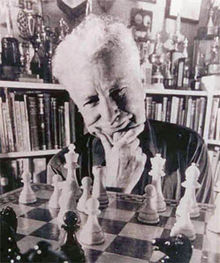
\includegraphics[width=0.19\textwidth]{ArpadElo}\hspace{1cm}

\includegraphics[width=0.18\textwidth]{Halo3}
}

Competition is central to our lives. It is an innate biological trait,
and the driving principle of many sports.\\[1ex]

In the Ancient Olympics (700 BC), the winners of the events were
admired and immortalised in poems and statues.\\[1ex]

Today in pretty much every sport there are player or team
rankings. (Football leagues, Poker tournament rankings, etc).\\[1ex]

We are going to focus on one example: \Blue{\emph{tennis players}},
in men singles games.\\[1ex]

We are going to keep in mind the goal of answering the following question:\\
\Blue{\emph{What is the probability that player 1 defeats player 2?}}
\end{frame}


\begin{frame}
\frametitle{The ATP ranking system for tennis players}
Men Singles ranking as of 28 December 2011:\\[2ex]

\centerline{\footnotesize
\begin{tabular}{l | r | c}
\Blue{Rank, Name \& Nationality}& \Blue{Points} & \Blue{Tournaments Played} \\
\hline
1 Djokovic, Novak (SRB)         & 13,675    & 19           \\
2 Nadal, Rafael (ESP)           & 9,575     & 20           \\
3 Federer, Roger (SUI)          & 8,170     & 19           \\
4 Murray, Andy (GBR)            & 7,380     & 19           \\
5 Ferrer, David (ESP)           & 4,880     & 23           \\
6 Tsonga, Jo-Wilfried (FRA)     & 4,335     & 25           \\
7 Berdych, Tomas (CZE)          & 3,700     & 24           \\
8 Fish, Mardy (USA)             & 2,965     & 24           \\
9 Tipsarevic, Janko (SRB)       & 2,595     & 28           \\
10 Almagro, Nicolas (ESP)       & 2,380     & 27           \\
11 Del Potro, Juan Martin (ARG) & 2,315     & 22           \\
12 Simon, Gilles (FRA)          & 2,165     & 28           \\
13 Soderling, Robin (SWE)       & 2,120     & 22           \\   
14 Roddick, Andy (USA)          & 1,940     & 20           \\
15 Monfils, Gael (FRA)          & 1,935     & 23           \\
16 Dolgopolov, Alexandr (UKR)   & 1,925     & 30           \\  
17 Wawrinka, Stanislas (SUI)    & 1,820     & 23           \\
18 Isner, John (USA)            & 1,800     & 25           \\   
19 Gasquet, Richard (FRA)       & 1,765     & 21           \\
20 Lopez, Feliciano (ESP)       & 1,755     & 28           
\end{tabular}
}
{\hfill\tiny ATP: Association of Tennis Professionals (\texttt{www.atpworldtour.com})}
\end{frame}


\begin{frame}
\frametitle{The ATP ranking system explained (to some degree)}

\begin{itemize}
\item Sum of points from best 18 results of the past 52 weeks.
\item Mandatory events: 4 Grand Slams, and 8 Masters 1000 Series events.
\item Best 6 results from International Events (4 of these must be 500 events).
\end{itemize}
Points breakdown for all tournament categories (2012):

\centerline{
{\scriptsize
\begin{tabular}{l| c| c| c| c| c| c| c| c| c }
& W&    F&      SF&     QF&     R16&    R32&    R64&    R128&   Q\\
\hline
Grand Slams&    2000&   1200&   720&    360&    180&    90&     45&     10&     25\\
\hline
Barclays ATP World Tour Finals & *1500\\
\hline                                                  
ATP World Tour Masters 1000 & 1000 & 600 & 360 & 180 & 90 & 45 & 10(25) & (10) & (1)25\\
\hline
ATP 500 & 500 & 300 & 180 & 90 & 45 & (20) &  &  & (2)20\\
\hline
ATP 250 & 250 & 150 & 90 & 45 & 20 & (5) &  &  & (3)12\\
\hline
Challenger 125,000 +H & 125 & 75 & 45 & 25 & 10 &  &  &  & 5\\
\hline
Challenger 125,000 & 110 & 65 & 40 & 20 & 9 &  &  &  & 5\\
\hline
Challenger 100,000 & 100 & 60 & 35 & 18 & 8 &  &  &  & 5\\
\hline
Challenger 75,000 & 90 & 55 & 33 & 17 & 8 &  &  &  & 5\\
\hline
Challenger 50,000 & 80 & 48 & 29 & 15 & 7 &  &  &  & 3\\
\hline
Challenger 35,000 +H & 80 & 48 & 29 & 15 & 6 &  &  &  & 3\\
\hline
Futures** 15,000 +H & 35 & 20 & 10 & 4 & 1 &  &  &  & \\
\hline
Futures** 15,000 & 27 & 15 & 8 & 3 & 1 &  &  &  & \\
\hline
Futures** 10,000 & 18 & 10 & 6 & 2 & 1 &  &  &  & \\
\hline
\end{tabular}
}
}

{\tiny
The Grand Slams are the Australian Open, the French Open, Wimbledon, and the US Open.\\
The Masters 1000 Tournaments are: Cincinnati, Indian Wells, Madrid,
Miami, Monte-Carlo, Paris, Rome, Shanghai, and Toronto.\\
The Masters 500 Tournaments are: Acapulco, Barcelona, Basel, Beijing, Dubai, Hamburg, 
Memphis, Rotterdam, Tokyo, Valencia and Washington.\\
The Masters 250 Tournaments are: Atlanta, Auckland, Bangkok, Bastad, Belgrade, Brisbane,
Bucharest, Buenos Aires, Casablanca, Chennai, Delray Beach, Doha,\\
Eastbourne, Estoril, Gstaad, Halle, Houston, Kitzbuhel, Kuala Lumpur, London, Los Angeles, Marseille, Metz, Montpellier, Moscow, Munich, Newport, Nice,\\
Sao Paulo, San Jose, 's-Hertogenbosch, St. Petersburg, Stockholm, Stuttgart, Sydney, Umag, Vienna, Vina del Mar, Winston-Salem, Zagreb and Dusseldorf.\\
}
\end{frame}


\begin{frame}
\frametitle{A laundry list of objections and open questions}

\centerline{\footnotesize
\begin{tabular}{l | r | c}
\Blue{Rank, Name \& Nationality}& \Blue{Points} \\
\hline
1 Djokovic, Novak (SRB)         & 13,675  \\
2 Nadal, Rafael (ESP)           & 9,575   \\
3 Federer, Roger (SUI)          & 8,170   \\
4 Murray, Andy (GBR)            & 7,380   \\
\end{tabular}
}

Some questions:
\begin{itemize}
\item Is a player ranked higher than another more likely to win?
\item What is the probability that Nadal defeats Djokovic?
\item \Blue{\emph{How much would you (rationally) bet on Nadal?}}
\end{itemize}

And some concerns:
\begin{itemize}
\item The points system ignores who you played against.
\item 6 out of the 18 tournaments don't need to be common to two players.
\end{itemize}

Other examples: Premier League. Meaningless intermediate results
throughout the season: doesn't say whom you played and whom you
didn't!
\end{frame}


\begin{frame}
\frametitle{Towards a probabilistic ranking system}

What we really want is to infer is a player's \Blue{\emph{skill}}.
\begin{itemize}
\item Skills must be comparable: a player of higher skill is more likely to win.
\item We want to do probabilistic inference of players' skills.
\item We want to be able to compute the probability of a game outcome.
\end{itemize}

A generative model for game outcomes:
\begin{enumerate}
\item Take two tennis players with known \Blue{\emph{skills}} ($w_i\in\mathbb{R}$)
\begin{itemize}
\item Player 1 with skill $w_1$.
\item Player 2 with skill $w_2$.
\end{itemize}
\item Compute the difference between the skills of Player 1 and Player 2:\\
\centerline{ $s = w_1 - w_2$}
\item Add noise ($n\sim\N(0,1)$) to account for \Red{\emph{performance}} inconsistency:\\
\centerline{$t = s + n$}
\item The game outcome is given by $y=\operatorname{sign}(t)$
\begin{itemize}
\item $y=+1$ means Player 1 wins.
\item $y=-1$ means Player 2 wins.
\end{itemize}
\end{enumerate}
\end{frame}


\begin{frame}
\frametitle{The likelihood in a picture}

\centerline{
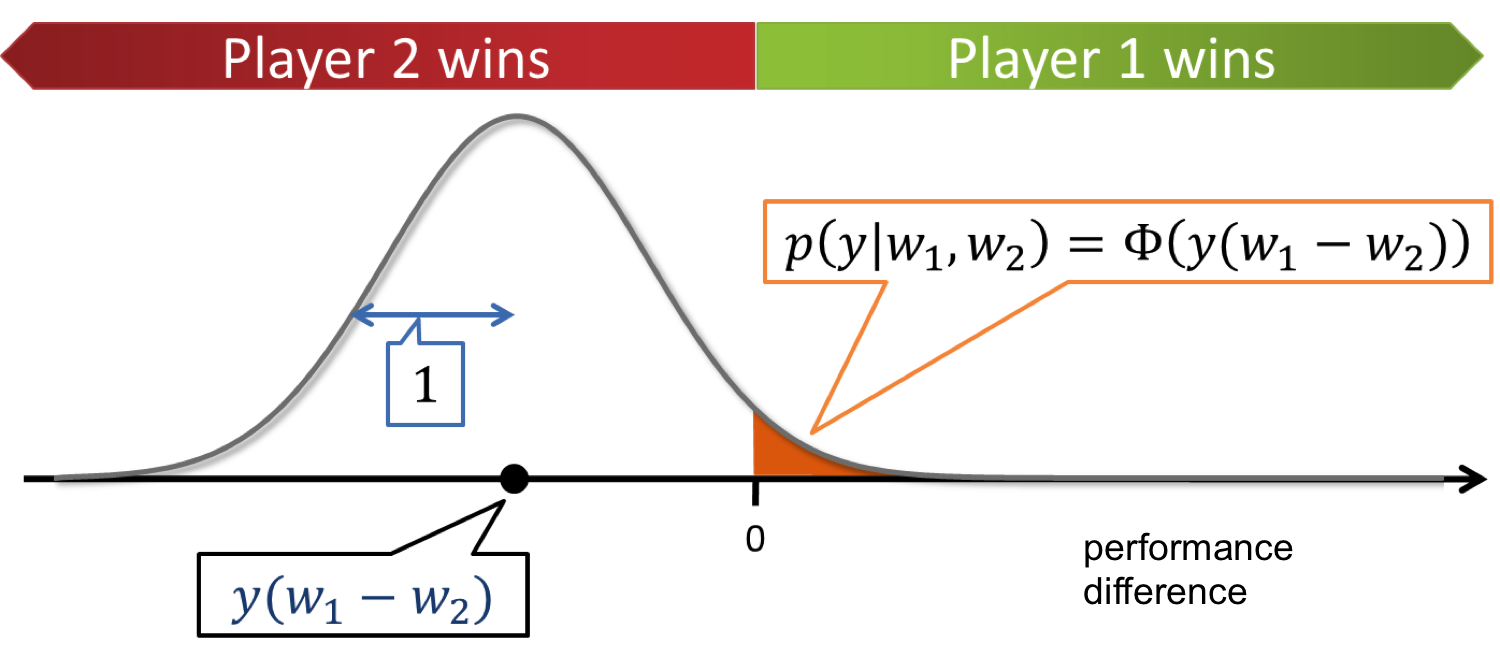
\includegraphics[width=\textwidth]{TrueSkillLikelihoodIntuition2}
}
\vskip -3ex
\[
t\;=\;w_1-w_2+n, \qquad p(t|w_1, w_2)\;=\;{\cal N}(t; w_1-w_2, 1).
\]
So, what is the probability that player 1 wins, given the skills $p(y=1|w_1,w_2)$?
\[
\begin{split}
&p(y=1|w_1,w_2)\;=\;p(t>0|w_1,w_2)\;=\;\Phi(w_1-w_2),\\
&\text{since\ \ }\Phi(x)\;=\;\int_{-\infty}^x {\cal N}(z; 0, 1)dz
\;=\;\int_0^\infty{\cal N}(z; x, 1)dz.
\end{split}
\]
\end{frame}


\begin{frame}
\frametitle{The Likelihood}
\begin{align*}
t &\;=\; w_1 - w_2 + n,\qquad y\;=\;\operatorname{sign}(t) \\
\Blue{p}\Blue{(y|w_1,w_2)}&= \int\!\!\int p(y|t)p(t|s)p(s|w_1,w_2)\mathrm{d}s\mathrm{d}t
= \int p(y|t)p(t|w_1,w_2)\mathrm{d}t\\
&= \Blue{\Phi(y(w_1-w_2))},
\end{align*}
where we have the little compactifying trick for binary variables $y=\pm 1$
\[
p(y=1|z)\;=\;\Phi(z)\;\Longrightarrow p(y=-1|z)\;=\;1-\Phi(z)\;=\;\Phi(-z)\;
\Longrightarrow\;p(y|z) = \Phi(yz).
\]
\centerline{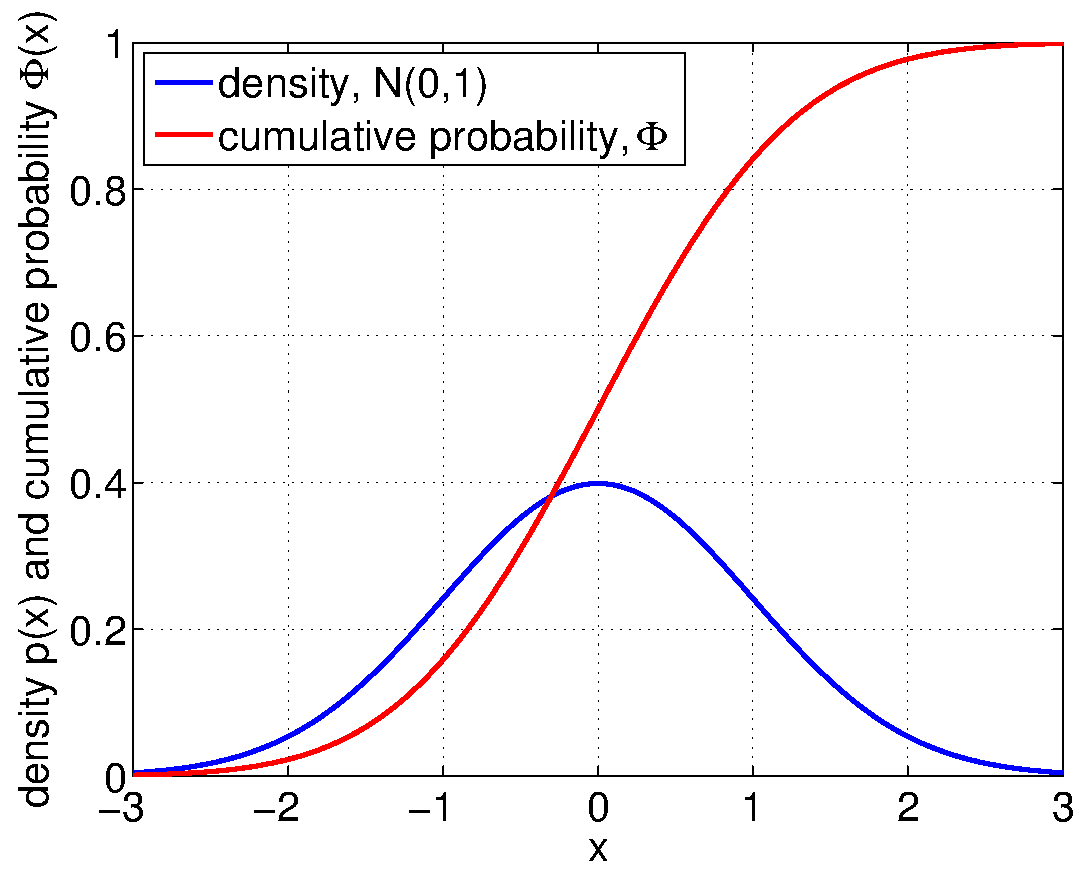
\includegraphics[width=0.38\textwidth]{gpdfcdf}}

\end{frame}

\begin{frame}
\frametitle{TrueSkill\texttrademark, a probabilistic skill rating system}

\parbox{0.30\textwidth}{
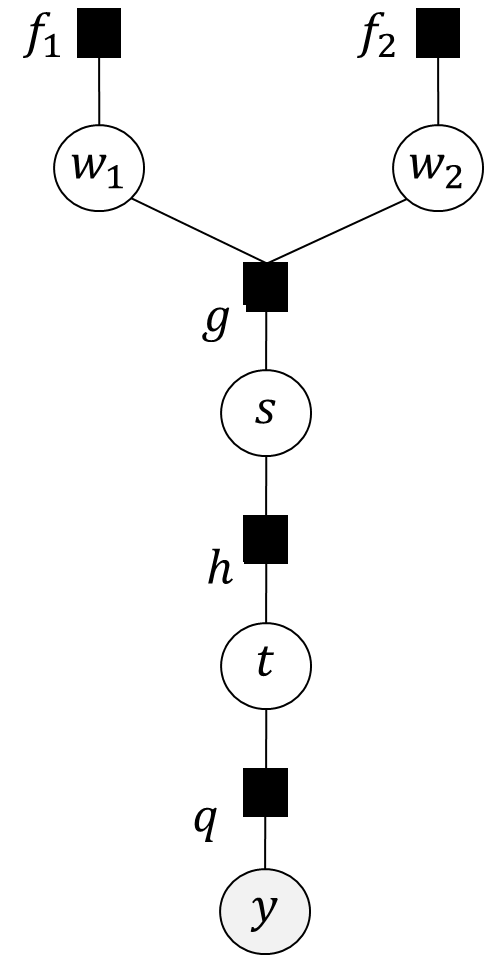
\includegraphics[width=0.3\textwidth]{TrueSkillFactorGraph}
}
\parbox{0.69\textwidth}{
\begin{itemize}
\item $w_1$ and $w_2$ are the skills of Players 1 and 2.\\
We treat them in a Bayesian way:
\[
\textrm{\Red{prior}\;\;\;\;\;\;\;\;\;\;\;\;\;\;}\Red{p(w_i)} = \N(w_i|\mu_i, \sigma_i^2)
\;\;\;\;\;\;\;\;\;\;\;\;\;\; 
\]
\item $s=w_1-w_2$ is the \emph{skill difference}.
\item $t\sim\N(t|s, 1)$ is the \emph{performance difference}.
\item  $y= \operatorname{sign}(t) $ is the \emph{game outcome}.
\item the \Blue{likelihood} is the probability of outcome given skills:
\[
\Blue{p(y|w_1,w_2)} = \int\!\!\int p(y|t)p(t|s)p(s|w_1,w_2)\mathrm{d}s\mathrm{d}t
\]
\item The \Green{posterior} over skills given the game outcome is:
\[
\Green{p(w_1,w_2|y)} = \frac{\Red{p(w_1)p(w_2)}\Blue{p(y|w_1,w_2)}}
{\int\!\!\int \Red{p(w_1)p(w_2)}\Blue{p(y|w_1,w_2)}\mathrm{d}w_1\mathrm{d}w_2}
\]
\end{itemize}
}
{\scriptsize TrueSkill\texttrademark: A Bayesian Skill Rating
System. Herbrich, Minka and Graepel, NIPS19, 2007.}
\end{frame}


\begin{frame}
\frametitle{An intractable posterior}

The joint posterior distribution over skills does not have a closed form:
\[
\Green{p(w_1,w_2|y)} = \frac{\Red{\N(w_1; \mu_1, \sigma_1^2)\N(w_2; \mu_2, \sigma_2^2)}
\Blue{\Phi(y(w_1-w_2))}}
{\int\!\!\int \Red{\N(w_1; \mu_1, \sigma_1^2)\N(w_2; \mu_2, \sigma_2^2)}
\Blue{\Phi(y(w_1-w_2))}\mathrm{d}w_1\mathrm{d}w_2}
\]

\begin{itemize}
\item $w_1$ and $w_2$ become correlated, the posterior does not factorise.
\item The posterior is no longer a Gaussian density function.
\end{itemize}
The normalising constant of the posterior, the prior over $y$ does have closed form:
\[
p(y) = \int\!\!\int \N(w_1; \mu_1, \sigma_1^2)\N(w_2; \mu_2, \sigma_2^2)
\Phi(y(w_1-w_2))\mathrm{d}w_1\mathrm{d}w_2 = 
\Phi\!\Big(\!\frac{y(\mu_1-\mu_2)}{\sqrt{1+\sigma_1^2+\sigma_2^2}}\!\Big)
\]
This is a \emph{smoother} version of the likelihood $p(y|w_1,w_2)$.\\
\hfill\Blue{\emph{Can you explain why?}}
\end{frame}


\begin{frame}
\frametitle{Joint posterior after several games}

Each player playes against multiple opponents, possibly multiple
times; what does the joint posterior look like?

\centerline{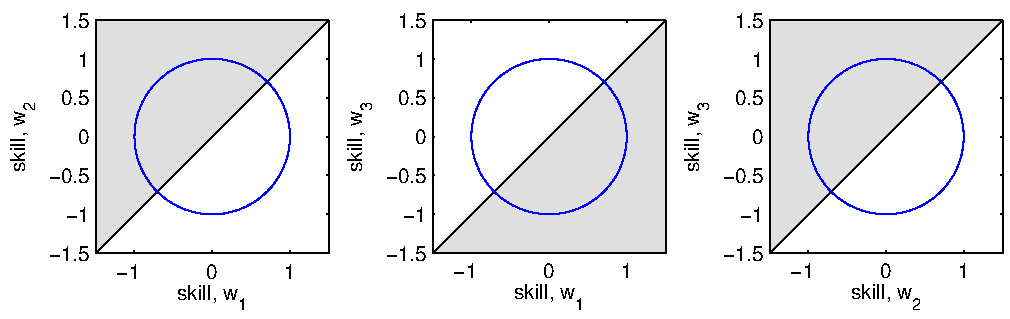
\includegraphics[width=\textwidth]{jp}}

The combined posterior is difficult to picture.

\hfill\Blue{\emph{How do we do inference with an ugly posterior like
    that?}}

\hfill\Blue{\emph{How do we predict the outcome of a match?}}
\end{frame}

\begin{frame}
\frametitle{Appendix: The likelihood in detail}

\begin{align*}
\Blue{p}&\Blue{(y|w_1,w_2)} = \int\!\!\int p(y|t)p(t|s)p(s|w_1,w_2)\mathrm{d}s\mathrm{d}t
= \int p(y|t)p(t|w_1,w_2)\mathrm{d}t\\
&= \int_{-\infty}^{+\infty}\!\! \delta(y-\operatorname{sign}(t))\N(t| w_1-w_2, 1
)\mathrm{d}t\\
&= \int_{-\infty}^{+\infty}\!\! \delta(1-\operatorname{sign}(y t))\N(y t| y(w_1-
w_2), 1)\mathrm{d}t\\
&= y \int_{-y\infty}^{+y\infty}\!\! \delta(1-\operatorname{sign}(z))\N(z| y(w_1-
w_2), 1)\mathrm{d}z
\;\;\;\;\;\;\;\;\;\;\;\;\, (\mathrm{use}\;\; z\equiv yt)\\
&= \int_{-\infty}^{+\infty}\!\! \delta(1-\operatorname{sign}(z))\N(z| y(w_1-w_2)
, 1)\mathrm{d}z\\
&= \int_{0}^{+\infty}\!\! \N(z| y(w_1-w_2), 1)\mathrm{d}z
= \int_{-\infty}^{y(w_1-w_2)} \!\!\!\!\!\!\!\!\!\!\!\!\N(x| 0, 1)\mathrm{d}x
\;\;\;\;\;\; (\mathrm{use}\; x\equiv y(w_1-w_2)-z)\\
&= \Blue{\Phi(y(w_1-w_2))}
\;\;\;\;\;\;\;\;\;\;\;\;\;\;\; 
\;\;\;\;\;\;\;\;\;\;\;\;\;\;\; 
\;\;\;\;\;\;\;\;\;\;\;\;\;\;\; 
\big(\mathrm{where}\; \Phi(a)=\int_{-\infty}^a \N(x| 0, 1)\mathrm{d}x\big)
\end{align*}

$\Phi(a)$ is the Gaussian cumulative distribution function, or `probit' function.

\end{frame}

\end{document}